% VLDB template version of 2020-08-03 enhances the ACM template, version 1.7.0:
% https://www.acm.org/publications/proceedings-template
% The ACM Latex guide provides further information about the ACM template

\documentclass[sigconf, nonacm]{acmart}
\usepackage[english]{babel}
\usepackage{tikz}
\usepackage{amsmath}
\usepackage{xspace}
\usepackage{makecell}
\usepackage{pifont}
\usepackage{amsfonts}
\usepackage{makecell}
\usepackage[font=small,labelfont=bf]{caption}
% inlined bib file
\usepackage{filecontents}
\usepackage{xurl}
\usepackage{listings}
\usepackage{minted}

\newcommand\sysname{\textsf{ElimDA}\xspace}
\newcommand\redbf{\bf\color{red}}
\renewcommand{\paragraph}[1]{\smallskip\noindent {\bf #1}}
\newcommand\blfootnote[1]{%
  \begingroup
  \renewcommand\thefootnote{}\footnote{#1}%
  \addtocounter{footnote}{-1}%
  \endgroup
}

%% The following content must be adapted for the final version
% paper-specific
\newcommand\vldbdoi{XX.XX/XXX.XX}
\newcommand\vldbpages{XXX-XXX}
% issue-specific
\newcommand\vldbvolume{14}
\newcommand\vldbissue{1}
\newcommand\vldbyear{2020}
% should be fine as it is
\newcommand\vldbauthors{\authors}
\newcommand\vldbtitle{\shorttitle}
% leave empty if no availability url should be set
\newcommand\vldbavailabilityurl{URL_TO_YOUR_ARTIFACTS}
% whether page numbers should be shown or not, use 'plain' for review versions, 'empty' for camera ready
\newcommand\vldbpagestyle{plain}

%-------------------------------------------------------------------------------
\begin{document}
%-------------------------------------------------------------------------------

%don't want date printed
\date{}

% make title bold and 14 pt font (Latex default is non-bold, 16 pt)
\title{Eliminating Double Amplifications of Hashing Indexes for Persistent Memory}
%for single author (just remove % characters)
\author{
  Paper ID: 98
} % end author

\maketitle

%-------------------------------------------------------------------------------
\section{Summary of Implementations}
%-------------------------------------------------------------------------------

We implement our proposed \sysname with C++.
We elaborate on the dependent software,
representative hash indexes, and testing tools as follows.

\paragraph{Dependent softwares:} the implementation of
\sysname relies on a suite of software, including
  {\tt ndctl}, {\tt ipmctl}, {\tt Intel PMWatch}, and {\tt PMDK},
which can be reached via the following URLs.

\begin{minted}{bash}
  $ wget https://github.com/pmem/ndctl
  $ wget https://github.com/intel/ipmctl
  $ wget https://github.com/intel/intel-pmwatch
  $ wget https://github.com/pmem/pmdk
\end{minted}

\paragraph{Representative hash indexes:}
we use four representative hash indexes for comparison, namely
CCEH \cite{Nam19}, Dash \cite{Lu20}, level hashing \cite{Zuo18} and clevel hashing \cite{Zuo20},
which can be downloaded via the following URLs.
Note that we used the PMDK version of the level hashing implemented by Dash and add uniqueness check to CCEH for index correctness.

\begin{minted}{bash}
  $ wget https://github.com/DICL/CCEH/tree/master/
  CCEH-PMDK
  $ wget https://github.com/pmdk/dash
  $ wget https://github.com/chenzhangyu/Clevel-Hashing
\end{minted}

\paragraph{Testing tools:} we employ {\tt YCSB} in our evaluation.
It can be reached via the following URL.

\begin{minted}{bash}
  $ wget https://github.com/brianfrankcooper/YCSB/
  releases/download/0.17.0/ycsb-0.17.0.tar.gz
\end{minted}

%-------------------------------------------------------------------------------
\section{Evaluation Details}
%-------------------------------------------------------------------------------

\paragraph{Hardware configurations:}
We conduct extensive experiments on a single machine
equipped with two 2.10\,GHz Intel Golden 5318Y CPUs
(with 24 cores in total), 128\,GB of DRAM memory and four
Optane PMem DIMMs of 200 series (128\,GB per DIMM and
512\,GB in total). The Optane PMem DIMMs are configured
in interleaved {AppDirect Mode, which are connected to one
processor. Figure~\ref{fig:processor} shows the major
hardware configurations of our testbed and
Figure~\ref{fig:pmem} shows detailed information
about the Optane PMem used in our evaluation.

\begin{figure}[t]
  \centering
  \hspace{-0.1in}
  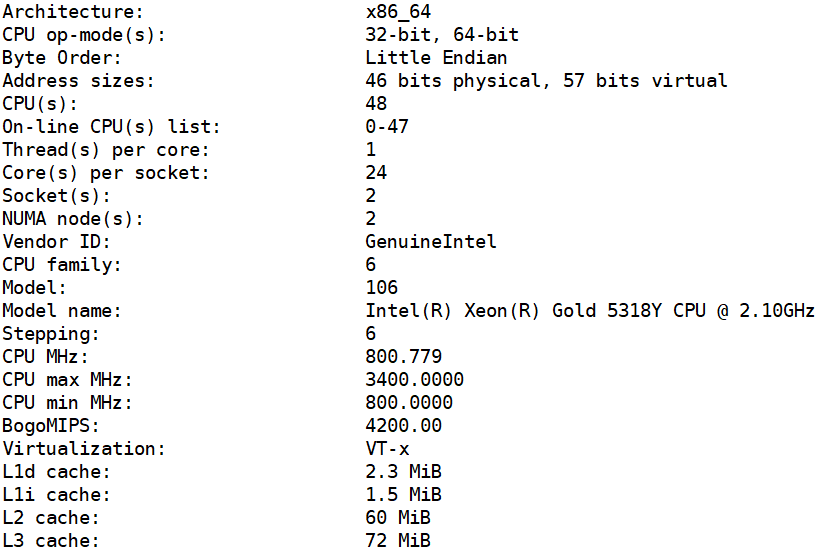
\includegraphics[width=8.5cm]{figures/hardware.png}
  \caption{Configurations of our testbed.}
  \label{fig:processor}
\end{figure}

\begin{figure}[t]
  \centering
  \hspace{-0.1in}
  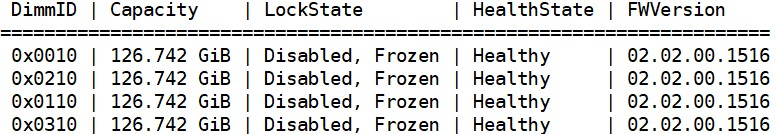
\includegraphics[width=8.5cm]{figures/PMem.jpg}
  \caption{The configurations of the Intel Optane PMem DIMMs of 200 series used in
    the evaluation.}
  \label{fig:pmem}
\end{figure}

We perform extensive testbed experiments, including (i) experiments to understand
the property of \sysname, and (ii) experiments to understand the sensitivity of \sysname.

\paragraph{Experiments with YCSB:}
We measure the access performance of \sysname, CCEH, Dash, level hashing, and clevel hashing using {\tt YCSB}.
We generate the workloads through {\tt YCSB} and then modify their format so that they can be used for testing.
We then use these workloads to test each hashing index.

The following script is an example of how to generate an insert-only workload using {\tt YCSB}:
\begin{minted}{bash}
  #!/bin/bash
  $ ycsb load basic -P uniformworkload > uniform/load.text
  $ ycsb run basic -P insertworkload > uniform/insert.text
\end{minted}

We run the following script to modify the format of workloads.
\begin{minted}{bash}
  #!/bin/bash
  $ dir=./uniform/load.txt
  $ sed -i '1,17d' $dir
  $ sed -i 's/READ usertable user/r /' $dir
  $ sed -i 's/INSERT usertable user/i /' $dir
  $ sed -i 's/UPDATE usertable user/u /' $dir
  $ sed -i 's/\[ field0=/ /' $dir
  $ sed -i 's/\ ]/ /' $dir
\end{minted}

After modifying the format, we measure the performance of all hashing indexes.
Due to space limits, we present the following script to evaluate \sysname.
The experiments with other hashing indexes are similar.
\begin{minted}{bash}
  #!/bin/bash
  dir=/mnt/pmem1-node0/pool1
  loadsize=50000000
  runsize=50000000
  FLAG='-mavx -mavx2 -mavx512f -mavx512bw -mavx512vl'

  g++ -O3 -std=c++17 -I./ -lrt -c -o src/ElimDA.o -g \
  src/ElimDA.cpp -DINPLACE -lpmemobj -lpmem \
  $FLAG -lprofiler -lunwind

  g++ -O3 -std=c++17 -I./ -lrt  -o bin/run_all_ycsb \
  -g src/run_all_ycsb.cpp src/ElimDA.o include/dlock.o  \
  -lpmemobj -lpmem -lpthread -DMULTITHREAD -lpqos

  outdir=ycsb_all
  for test in 1 2 3 4
  do
      for oper in "w50r50.txt"
      do
          for num in 1 2 4 8 16 24
          do
              echo " " >> $outdir
              echo "test zipfian  "$num" "$oper >> $outdir
              ycsb_dir="../ycsb/zipfian/"$oper
              load_dir="../ycsb/zipfian/load.txt"
              rm -rf $dir

              numactl -N 0 -m 0 \
              ./bin/run_all_ycsb $dir $loadsize $runsize
              $num $ycsb_dir $load_dir
              |grep -a -E "num|Ops|Start" >> $outdir
          done
      done
  done
\end{minted}

\paragraph{Experiments on Sensitivity:}
We also use the impact of the P-bucket size (Exp\#12)
as an example to clarify how we assess
the performance of \sysname.
Other experiments are similar.
\begin{minted}{bash}
  #!/bin/bash
  dir=/mnt/pmem1-node0/pool1
  num=1
  loadsize=50000000
  FLAG='-mavx -mavx2 -mavx512f -mavx512bw -mavx512vl'
  outdir=./sendata
  srcdir=./sensitive.cpp
  for testnum in 1 2 3 4 5
  do
      for sbucketsize in 64 128 256 512 1024
      do
          sed -i '27d' ./src/ElimDA.h
          sed -i '27i #define S_Bucket_Size '\
          $sbucketsize'' ./src/ElimDA.h
          rm -rf $dir

          g++ -O3 -std=c++17 -I./ -lrt -c \
          -o src/ElimDA.o -g src/ElimDA.cpp \
          -DINPLACE -lpmemobj -lpmem \
          $FLAG -lprofiler -lunwind

          g++ -O3 -std=c++17 -I./ -lrt  \
          -o bin/multi_threaded_ElimDA -g \
          src/test.cpp src/ElimDA.o include/dlock.o \
          -lpmemobj -lpmem -lpthread \
          -DMULTITHREAD -lpqos

          numactl -N 0 -m 0 \
          ./bin/multi_threaded_ElimDA $dir $loadsize $num \
          |grep -a "Ops/sec" >> $outdir
      done
      sed -i '27d' ./src/ElimDA.h
      sed -i '27i #define S_Bucket_Size 256' ./src/ElimDA.h
  done
\end{minted}

%The output is in figure \ref{fig:slmdbycsb}.

\bibliographystyle{plain}
\bibliography{paper}
%%%%%%%%%%%%%%%%%%%%%%%%%%%%%%%%%%%%%%%%%%%%%%%%%%%%%%%%%%%%%%%%%%%%%%%%%%%%%%%%
\end{document}
%%%%%%%%%%%%%%%%%%%%%%%%%%%%%%%%%%%%%%%%%%%%%%%%%%%%%%%%%%%%%%%%%%%%%%%%%%%%%%%%

